%%%%%%%%%%%%%%%%%%%%%%%%%%%%%%%%%%%%%%%%%
% Jacobs Landscape Poster
% LaTeX Template
% Version 1.1 (14/06/14)
%
% Created by:
% Computational Physics and Biophysics Group, Jacobs University
% https://teamwork.jacobs-university.de:8443/confluence/display/CoPandBiG/LaTeX+Poster
% 
% Further modified by:
% Nathaniel Johnston (nathaniel@njohnston.ca)
%
% This template has been downloaded from:
% http://www.LaTeXTemplates.com
%
% License:
% CC BY-NC-SA 3.0 (http://creativecommons.org/licenses/by-nc-sa/3.0/)
%
%%%%%%%%%%%%%%%%%%%%%%%%%%%%%%%%%%%%%%%%%

%----------------------------------------------------------------------------------------
%	PACKAGES AND OTHER DOCUMENT CONFIGURATIONS
%----------------------------------------------------------------------------------------

\documentclass[final, 14pt]{beamer}

\usepackage[scale=1.24]{beamerposter} % Use the beamerposter package for laying out the poster

\usetheme{confposter} % Use the confposter theme supplied with this template

\setbeamercolor{block title}{fg=Mahogany,bg=white} % Colors of the block titles
\setbeamercolor{block body}{fg=black,bg=white} % Colors of the body of blocks
\setbeamercolor{block alerted title}{fg=white,bg=Mahogany} % Colors of the highlighted block titles
\setbeamercolor{block alerted body}{fg=black,bg=dblue!10} % Colors of the body of highlighted blocks
% Many more colors are available for use in beamerthemeconfposter.sty

%-----------------------------------------------------------
% Define the column widths and overall poster size
% To set effective sepwid, onecolwid and twocolwid values, first choose how many columns you want and how much separation you want between columns
% In this template, the separation width chosen is 0.024 of the paper width and a 4-column layout
% onecolwid should therefore be (1-(# of columns+1)*sepwid)/# of columns e.g. (1-(4+1)*0.024)/4 = 0.22
% Set twocolwid to be (2*onecolwid)+sepwid = 0.464
% Set threecolwid to be (3*onecolwid)+2*sepwid = 0.708

\newlength{\sepwid}
\newlength{\onecolwid}
\newlength{\twocolwid}
\newlength{\threecolwid}
\setlength{\paperwidth}{48in} % A0 width: 46.8in
\setlength{\paperheight}{36in} % A0 height: 33.1in
\setlength{\sepwid}{0.024\paperwidth} % Separation width (white space) between columns
\setlength{\onecolwid}{0.22\paperwidth} % Width of one column
\setlength{\twocolwid}{0.464\paperwidth} % Width of two columns
\setlength{\threecolwid}{0.708\paperwidth} % Width of three columns
\setlength{\topmargin}{-0.5in} % Reduce the top margin size
%-----------------------------------------------------------

\usepackage{graphicx}  % Required for including images

\usepackage{booktabs} % Top and bottom rules for tables

\usepackage{hyperref}

\usepackage{tikz}

\usepackage{mdframed}

%----------------------------------------------------------------------------------------
%	TITLE SECTION 
%----------------------------------------------------------------------------------------

\title{NBA Predictions}% Poster title

\author{Lee Richardson, Daren Wang, Xiaofeng Yu, Chi Zhang} % Author(s)

\institute{Carnegie Mellon University} % Institution(s)


%----------------------------------------------------------------------------------------

\begin{document}
\addtobeamertemplate{headline}{} 
{\begin{tikzpicture}[remember picture, overlay]
     \node [anchor=north west, inner sep=3cm]  at (current page.north west)
     {
\includegraphics[height=5cm]{nba.jpg}};
  \end{tikzpicture}}

\begin{document}
\addtobeamertemplate{headline}{} 
{\begin{tikzpicture}[remember picture, overlay]
     \node [anchor=north east, inner sep=3cm]  at (current page.north east)
     {
\includegraphics[height=5cm]{nba.jpg}};
  \end{tikzpicture}}


\addtobeamertemplate{block end}{}{\vspace*{2ex}} % White space under blocks
\addtobeamertemplate{block alerted end}{}{\vspace*{2ex}} % White space under highlighted (alert) blocks

\setlength{\belowcaptionskip}{2ex} % White space under figures
\setlength\belowdisplayshortskip{2ex} % White space under equations

\begin{frame}[t] % The whole poster is enclosed in one beamer frame

\begin{columns}[t] % The whole poster consists of three major columns, the second of which is split into two columns twice - the [t] option aligns each column's content to the top

\begin{column}{\sepwid}\end{column} % Empty spacer column

\begin{column}{\onecolwid} % The first column

%----------------------------------------------------------------------------------------
%	OBJECTIVES
%----------------------------------------------------------------------------------------

\begin{block}{Introduction and Goals}

\begin{itemize}

  \item The goal of this project was to predict the outcomes of NBA basketball games as accurately as possible

  \item Using game predictions, we can create a distribution of how many games each team is expected to win over the course of a season and compare with other projection systems. 

  \item We also looked at which features were the most important in terms of accurately predicting games. 

\end{itemize}

\end{block}


%----------------------------------------------------------------------------------------
% Data
%----------------------------------------------------------------------------------------

\begin{block}{Data}

Data collection and processing was a large portion of our project. We used web crawlers in the R and Python languages to extract data ftom three seperate data sources:

\begin{itemize}

  \item ESPN.com

  \item Basketball-Reference.com

  \item stats-for-the-nba.appspot.com

\end{itemize}

And then used ETL and merging techniques to load them all into an SQLite database. 

\begin{figure}
  \centering
	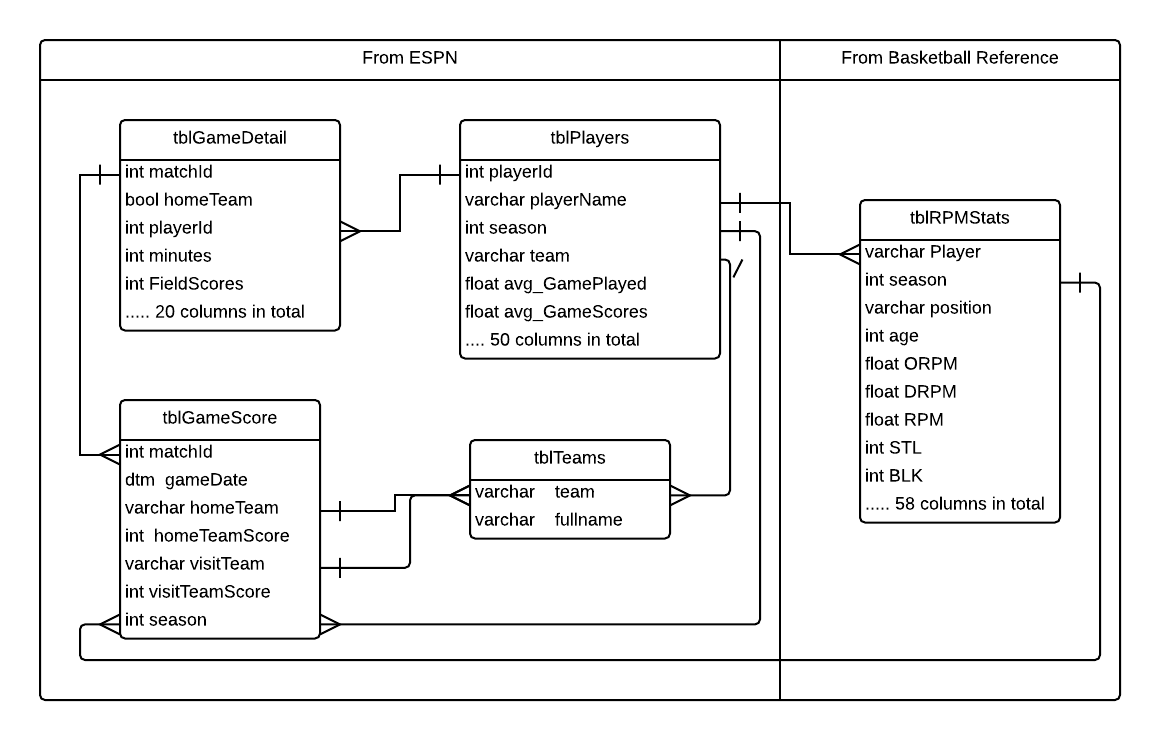
\includegraphics[width=25cm, height=20cm]{sqliteERDiagram.png}
  \caption{Entity-Relationship graph for SQLite database. The database follows the third normal form to ensure there is no redundancy. The lines between tables indicate the primary-foreign key relationship between dataset entities. }
  \label{fig:database}
\end{figure}

We have made our database publically available at \\

\url{https://github.com/leerichardson/game_simulation/blob/master/data/nba/nba.db}

\end{block}

%%%%%%%%%%%% CONTACT INFO %%%%%%%%%%%%%%%%%%%%%

\begin{alertblock}{Real Plus Minus (RPM)}

Throughout the poster we will refer to a feature called RPM. This is a new statistic which measures a player's estimated impact on efficiency per 100 possessions. It has become widely adopted in the basketball analytics community as the best measure of how good each individual player is both on offense and defense. 

\end{alertblock}


\end{column} % End of the first column

%----------------------------------------------------------------------------------------
% END OF COLUMN ONE
%----------------------------------------------------------------------------------------


\begin{column}{\sepwid}\end{column} % Empty spacer column

\begin{column}{\twocolwid} % Begin a column which is two columns wide (column 2)

\begin{columns}[t,totalwidth=\twocolwid] % Split up the two columns wide column

\begin{column}{\onecolwid}\vspace{-.6in} % The first column within column 2 (column 2.1)

%----------------------------------------------------------------------------------------
%	Data
%----------------------------------------------------------------------------------------

\begin{block}{Features}

\par Our final dataset had 44 different features, most of which were weighted averages for each team based on last seasons statistics. We also had features which exclusively considered the team performance in the previous season, but of course this does not account for player movement. 

\begin{figure}
  \centering
  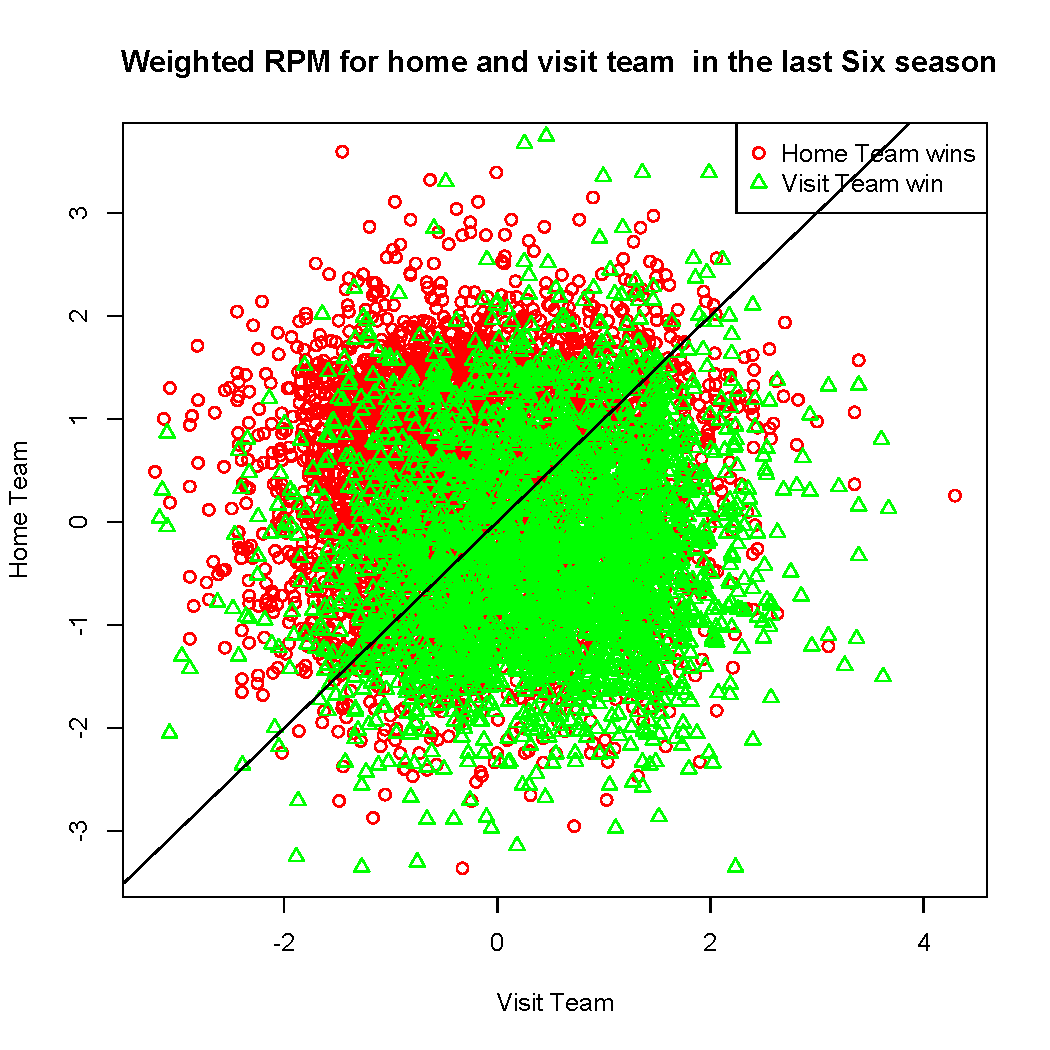
\includegraphics[width=25cm, height=25cm]{linear_seperable.pdf}
  \caption{This plot shows Home and Away weighted RPM for each of the games in our dataset. 
  This shows that our dataset is fairly messy, and certainly not linearly seperable. }
  \label{fig:features}
\end{figure}

\end{block}


\begin{block}{Feature Selection}

In order to choose which features were the most important, we used model selection techniques such as AIC. The following table shows the residual deviance of a logistic regression model if we were only to choose one covariate as a predictor. 

\begin{table}[h]

  \begin{mdframed}
  \begin{tabular}{lllll}
  \textbf{Feature} & \textbf{Deviance} \\
  \hline
  RPM Weight Away \vline & 9140.5 \\
  RPM Weight Home & 9160.6 \\
  Weighted Minutes & 9264.2 \\
  ORPM Weight Home & 9303.3 \\
  ORPM Weight Away & 9310.8 \\
  DRPM Weight Away & 9329.1 \\
  DRPM Weight Home & 9358.2 \\
  Previous Year Score Differential Home & 9376.9 \\
  Weighted Assists & 9384.7 \\
  Previous year Score Differential Away & 9389.6 \\
  \end{tabular}
  \end{mdframed}

\caption {This shows which single feature enhanced our model fit the most. Anything ending with \textttt{"RPM"} means Real Plus Minus, a new stat which is widely recognized as our best way to characterize the quality of which is quite clearly a superior predictor of performance compared with our othr features. }
\end{table}

\end{block}

%----------------------------------------------------------------------------------------

\end{column} % End of column 2.1

\begin{column}{\onecolwid}\vspace{-.6in} % The second column within column 2 (column 2.2)

%----------------------------------------------------------------------------------------
%	Geography
%----------------------------------------------------------------------------------------

\begin{block}{Algorithms}

\begin{figure}
  \centering
  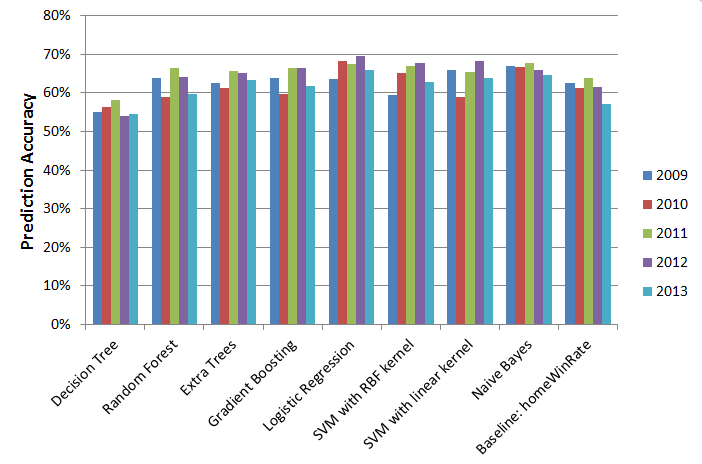
\includegraphics[width=28cm, height=30cm]{algorithms.png}
  \caption{This plot shows the test error for our different algorithms in all of our years. From this, we see that Naive Bayes and Logistic Regression gave us the best overall test error. For each testing year, we used all the previous years as training data. }
  \label{fig:algorithms}
\end{figure}


\begin{figure}
  \centering
  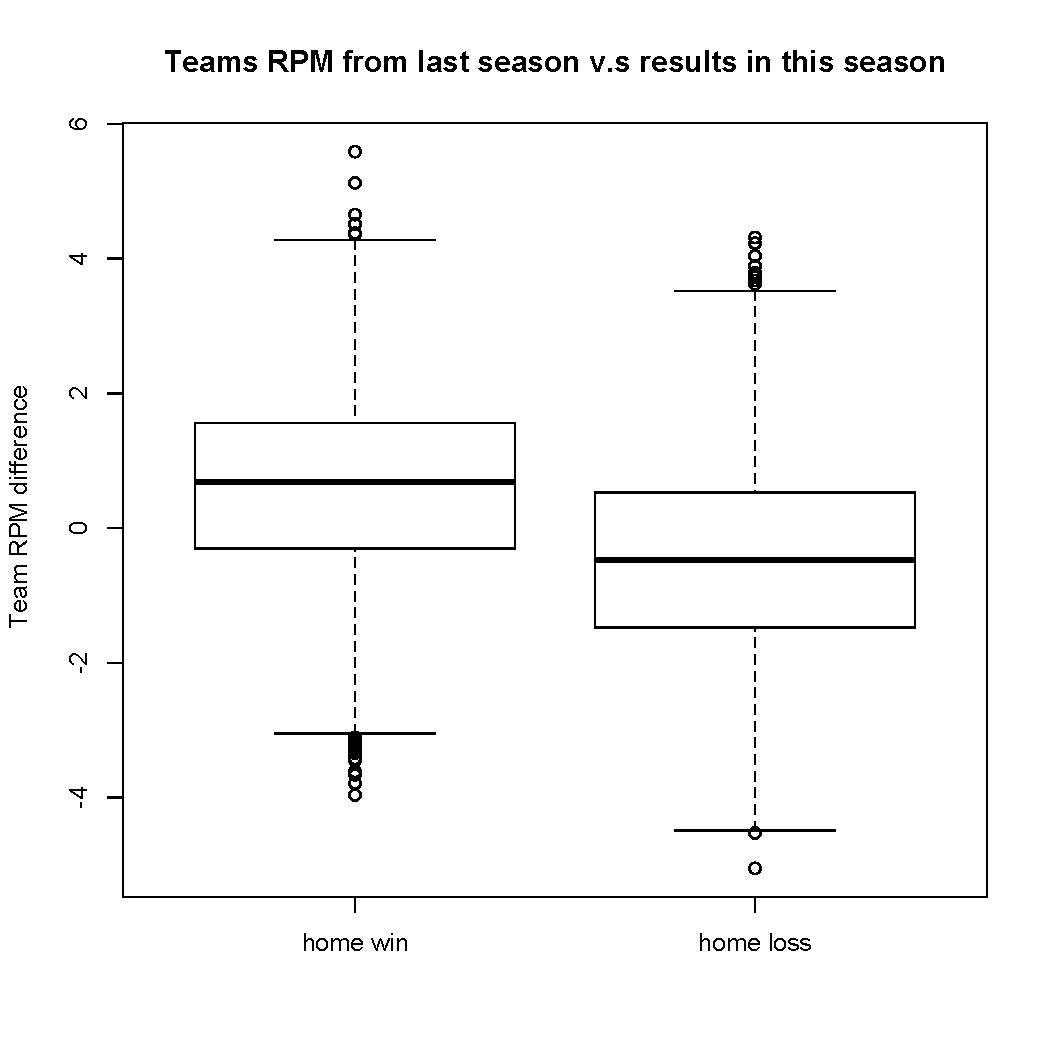
\includegraphics[width=25cm, height=25cm]{rpm_boxplot.pdf}
  \caption{This shows the Difference in RPM between the home and away team in wins and losses. It's clear there is some signal here, as the difference in RPM is much larger in wins compared with losses}
  \label{fig:rpm_dif}
\end{figure}

\end{block}

%----------------------------------------------------------------------------------------

\end{column} % End of column 2.2

\end{columns} % End of the split of column 2 - any content after this will now take up 2 columns width

\end{column} % End of the second column

%----------------------------------------------------------------------------------------
% END OF THE SECOND COLUMN
%----------------------------------------------------------------------------------------

\begin{column}{\sepwid}\end{column} % Empty spacer column

\begin{column}{\onecolwid} % The third column

%----------------------------------------------------------------------------------------
%	Simulations
%----------------------------------------------------------------------------------------

\begin{block}{Simulations}

\begin{figure}
  \centering
  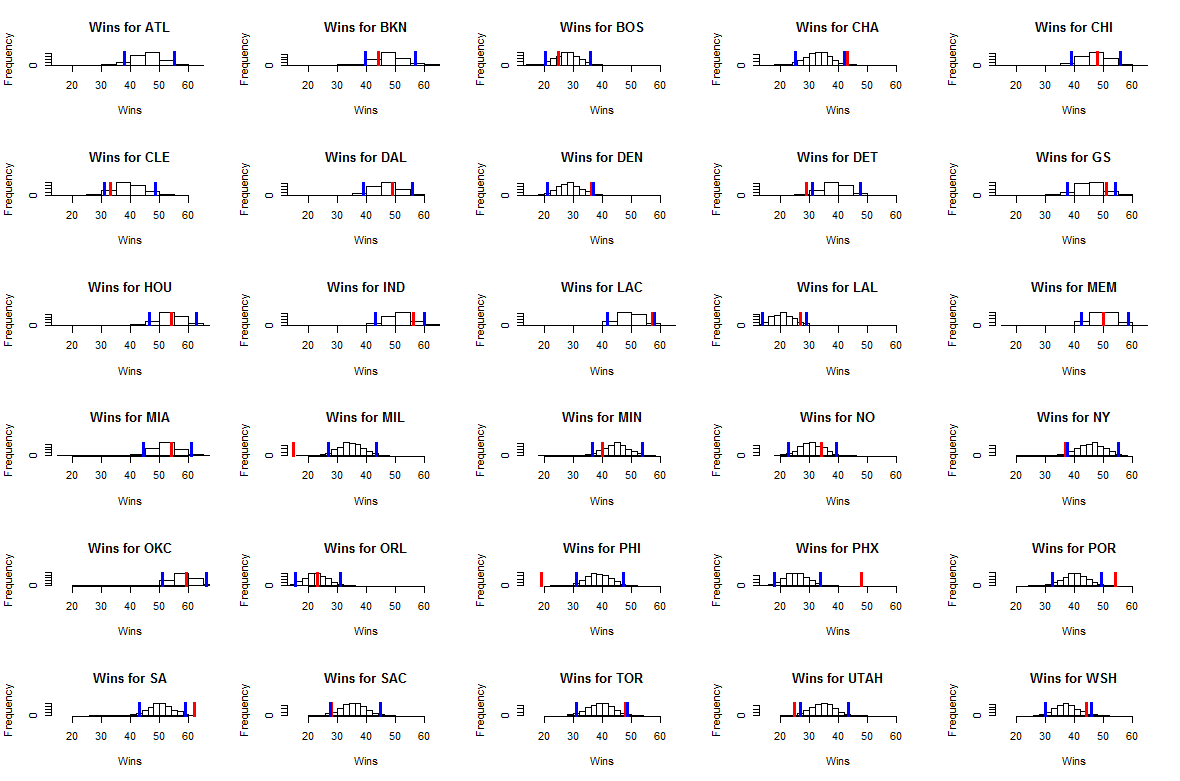
\includegraphics[width=30cm, height=35cm]{season_wins.png}
  \caption{Results from simulating the 2013 NBA season 1000 times, using probabilities from our best Logistic regression model. The blue lines represent our confidence intervals whereas the Red lines represent the actual number of wins for each team. Our simulations trapped the true number of wins in 70 \% of our intervals.}
  \label{fig:simulations}
\end{figure}

Our algorithms gave us probabilities that each team would win, one natural thing to do was to use these probabilities to simulate the season many times, and look at the distribution of wins. Our projections were in the top 15 in accuracy compared with many other projection systems. 

\end{block}

%----------------------------------------------------------------------------------------
%	CONCLUSION & Future Work
%----------------------------------------------------------------------------------------

\begin{block}{Conclusion and Future Work}

\begin{itemize}

  \item One of the first things we noticed is that on average, home teams win about 60\% of games. So just naively picking the home team without any information on how good the teams are gives a decent test error. 

  \item From this, the question then becomes how much better does the away team have to be in order to pick them to win the game. We found that Weighted Adjusted Plus minus (WAPM)was the best indicator of how good a team is. 

  \item In the future, we would like our WAPM to include more than just the previous season, and be a projection using more information. Also, we think that using current season data as a feature would be helpful and allow for predictions in the second half of the year to be stronger. 

\end{itemize}

\end{block}

%----------------------------------------------------------------------------------------

\end{column} % End of the third column

\end{columns} % End of all the columns in the poster

\end{frame} % End of the enclosing frame

\end{document}
